\subsection{ Winkeltreue Lambert Projektion}
\label{sec:lamwink}
Die winkeltreue Lambert Projektion ist winkeltreu. Die Längenkreise werden als Geraden dargestellt.
Die winkeltreue Lambert Projektion ist eine Kegelprojektion. 

Formel:\\
 \begin{eqnarray*}
 \mathcal{X}& = &\rho \sin ( n(\lambda -\lambda _0) )\\
 \mathcal{Y}& = &\rho _0-\rho \cos (n(\lambda - \lambda _0))\\
 \rho & = &F\cot ^n(\frac{1}{4}\pi + \frac{1}{2}\varphi)\\
 n& = &\dfrac{\ln (\cos \varphi _1 \sec \varphi _2)}{\ln (\tan (\frac{1}{4}\pi +\frac{1}{2}\varphi _2)\cot (\frac{1}{4}\pi + \frac{1}{2}\varphi _1))}\\
 F& = &\dfrac{\cos \varphi _1 \tan ^n(\frac{1}{4}\pi +\frac{1}{2}\varphi _1)}{n}
 \end{eqnarray*}\\
 
\begin{figure}[hbtp]
\centering
 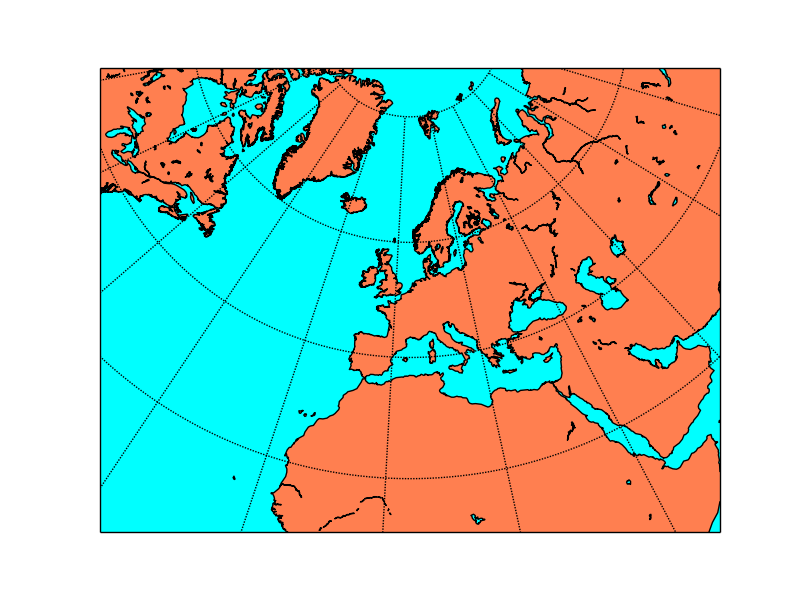
\includegraphics[scale=0.5,origin=c]{/Users/student/seminar/Kartendarstellungen/seminar/lcc} \caption{Winkeltreue Lambert-Projektion}
\end{figure}
\newpage 